\chapter{Mise en Œuvre du Sprint 1 : Configuration de l'Environnement de Développement et Authentification}

\section{Introduction}

Dans le cadre du sprint 1, l'équipe s'est concentrée sur la configuration de l'environnement de développement et la mise en place du système d'authentification pour l'application d'analyse de sentiments des commentaires sur Hespress. Ce sprint constitue la fondation technique de notre stack technologique complète utilisant Next.js pour le front-end, FastAPI pour le back-end, et Keycloak pour l'authentification. Voici un aperçu des activités réalisées durant cette période, qui ont permis d'établir les bases solides de l'infrastructure de développement.

L'objectif principal de ce premier sprint était de mettre en place l'environnement de développement complet (Next.js, FastAPI, Spring Gateway), de configurer le système d'authentification via Keycloak, et de valider l'intégration entre ces composants. Cette approche méthodique nous a permis de minimiser les risques techniques tout en garantissant une progression structurée du projet.

\section{Le Backlog du Sprint 1}

Le sprint 1 a été organisé autour de user stories prioritaires axées sur la configuration de l'environnement de développement et l'authentification. Chaque user story a été accompagnée de critères d'acceptation clairs pour garantir la qualité et la conformité aux attentes.

\subsection{User Story 1.1 : Configuration de l'environnement Next.js}

\textbf{En tant que} développeur front-end \\
\textbf{Je veux} configurer l'environnement de développement Next.js \\
\textbf{Afin de} disposer d'une interface utilisateur moderne et réactive

\textbf{Critères d'acceptation :}
\begin{itemize}
    \item Le projet Next.js est initialisé avec TypeScript
    \item Les dépendances UI nécessaires sont installées (Tailwind CSS, shadcn/ui)
    \item La structure de dossiers est organisée selon les bonnes pratiques
    \item L'environnement de développement est fonctionnel avec hot-reloading
\end{itemize}

\subsection{User Story 1.2 : Configuration de l'environnement FastAPI}

\textbf{En tant que} développeur back-end \\
\textbf{Je veux} configurer l'environnement de développement FastAPI \\
\textbf{Afin de} disposer d'une API performante pour le traitement des données

\textbf{Critères d'acceptation :}
\begin{itemize}
    \item L'environnement FastAPI est configuré et opérationnel
    \item La base de données PostgreSQL est connectée
    \item Redis est configuré pour le cache
    \item La documentation API automatique est accessible
\end{itemize}

\subsection{User Story 1.3 : Configuration du Spring Gateway}

\textbf{En tant que} développeur DevOps \\
\textbf{Je veux} configurer Spring Cloud Gateway \\
\textbf{Afin de} centraliser le routage et la sécurité des microservices

\textbf{Critères d'acceptation :}
\begin{itemize}
    \item Spring Gateway est configuré et déployé
    \item Le routage vers FastAPI est fonctionnel
    \item La configuration de base de sécurité est en place
    \item Les métriques et monitoring sont activés
\end{itemize}

\subsection{User Story 1.4 : Intégration de Keycloak pour l'authentification}

\textbf{En tant qu'} utilisateur \\
\textbf{Je veux} m'authentifier de manière sécurisée \\
\textbf{Afin d'} accéder aux fonctionnalités de l'application

\textbf{Critères d'acceptation :}
\begin{itemize}
    \item Keycloak est déployé et configuré
    \item Les realms et clients sont créés
    \item L'intégration avec Next.js est fonctionnelle
    \item L'intégration avec FastAPI via Spring Gateway est opérationnelle
\end{itemize}

\section{Configuration de l'Environnement de Développement}

Le Sprint 1 a été consacré à la mise en place complète de l'environnement de développement utilisant Next.js, FastAPI, Spring Gateway, PostgreSQL, Redis et Keycloak pour l'authentification.

\subsection{Choix Technologiques}

\subsubsection{Next.js pour le Front-end}

Next.js a été choisi comme framework front-end pour ses capacités de rendu hybride (SSR/SSG) et son écosystème riche. Il offre une excellente expérience développeur et des performances optimales pour les applications web modernes.

\textbf{Avantages :}
\begin{itemize}
    \item Rendu côté serveur (SSR) et génération statique (SSG)
    \item Optimisations automatiques (images, fonts, bundle)
    \item Router intégré avec navigation côté client
    \item Support TypeScript natif et hot-reloading
\end{itemize}

\subsubsection{FastAPI pour le Back-end}

FastAPI a été choisi comme framework backend pour sa performance exceptionnelle et sa facilité d'intégration avec les modèles de machine learning. Il permet de créer des APIs RESTful rapidement tout en maintenant des performances élevées.

\textbf{Avantages :}
\begin{itemize}
    \item Performance élevée avec support asynchrone
    \item Documentation automatique avec OpenAPI/Swagger
    \item Validation automatique des données avec Pydantic
    \item Intégration native avec les bibliothèques ML Python
\end{itemize}

\subsubsection{Spring Cloud Gateway}

Spring Gateway a été choisi comme API Gateway pour centraliser la gestion des requêtes et assurer la sécurité entre les microservices.

\textbf{Avantages :}
\begin{itemize}
    \item Routage intelligent des requêtes
    \item Load balancing automatique
    \item Intégration native avec Keycloak
    \item Monitoring et métriques intégrés
\end{itemize}

\subsubsection{PostgreSQL et Redis}

PostgreSQL a été sélectionné comme base de données principale pour sa robustesse et ses fonctionnalités avancées. Redis complète l'architecture en tant que solution de cache distribué.

\textbf{Avantages PostgreSQL :}
\begin{itemize}
    \item Support des types de données JSON
    \item Performances élevées pour les requêtes complexes
    \item Extensibilité et fonctions de recherche full-text
    \item Compatibilité ACID complète
\end{itemize}

\textbf{Avantages Redis :}
\begin{itemize}
    \item Cache en mémoire ultra-rapide
    \item Support des structures de données avancées
    \item Persistance configurable
    \item Pub/Sub pour les notifications temps réel
\end{itemize}

\subsubsection{Keycloak pour l'Authentification}

Keycloak a été choisi comme solution IAM (Identity and Access Management) pour gérer l'authentification et l'autorisation de manière centralisée.

\textbf{Avantages :}
\begin{itemize}
    \item Gestion complète des identités et accès
    \item Support des protocoles standards (OAuth 2.0, OpenID Connect)
    \item Interface d'administration complète
    \item Intégration facilitée avec les frameworks modernes
\end{itemize}

\subsection{Justification des Choix}

Le choix de cette stack technologique répond à trois exigences importantes du projet :

\textbf{Expérience utilisateur moderne :} Next.js offre une interface utilisateur réactive et performante, essentielle pour l'adoption de l'application par les utilisateurs finaux.

\textbf{Architecture scalable :} L'architecture microservices avec Spring Gateway permet de faire évoluer indépendamment chaque composant selon les besoins de charge.

\textbf{Sécurité centralisée :} Keycloak assure une gestion robuste et centralisée de l'authentification et des autorisations, conforme aux standards de sécurité.

\subsection{Conclusion}

Le choix des technologies pour le Sprint 1 a été guidé par la recherche de solutions modernes, performantes et scalables. Cette combinaison technologique constitue une base solide pour le développement d'un système d'analyse robuste et évolutif, tout en garantissant une excellente expérience utilisateur et une sécurité optimale.

\section{Analyse et Conception}

\subsection{Description Textuelle}

Le développement du sprint 1 s'est articulé autour de plusieurs phases clés axées sur la configuration et l'intégration :

\textbf{Configuration de l'environnement Next.js :} L'équipe a initialisé le projet front-end avec Next.js 14, configuré TypeScript, et intégré Tailwind CSS pour le styling. La structure de dossiers a été organisée selon les bonnes pratiques avec des composants réutilisables et une architecture modulaire.

\textbf{Configuration de l'environnement FastAPI :} Le backend a été configuré avec FastAPI, incluant la connexion à PostgreSQL via SQLAlchemy, l'intégration de Redis pour le cache, et la mise en place de la documentation automatique. Les modèles de données de base ont été définis avec Pydantic.

\textbf{Déploiement de Spring Gateway :} L'API Gateway a été configuré pour router les requêtes entre le front-end et le back-end, avec une configuration de base pour la sécurité et le monitoring. Les routes et filtres ont été définis pour une gestion centralisée du trafic.

\textbf{Intégration de Keycloak :} Le serveur d'authentification a été déployé avec la configuration des realms, clients, et utilisateurs de test. L'intégration avec Next.js a été réalisée via NextAuth.js, et la sécurisation des APIs FastAPI a été mise en place via les tokens JWT.

\textbf{Tests d'intégration :} Des tests d'intégration ont été mis en place pour valider le bon fonctionnement du flux d'authentification complet, depuis la connexion utilisateur jusqu'à l'accès aux APIs sécurisées. Cela a permis de détecter et corriger rapidement les problèmes de configuration.

\subsection{Diagramme de Cas d'Utilisation du Sprint 1}

\begin{figure}[H]
\centering
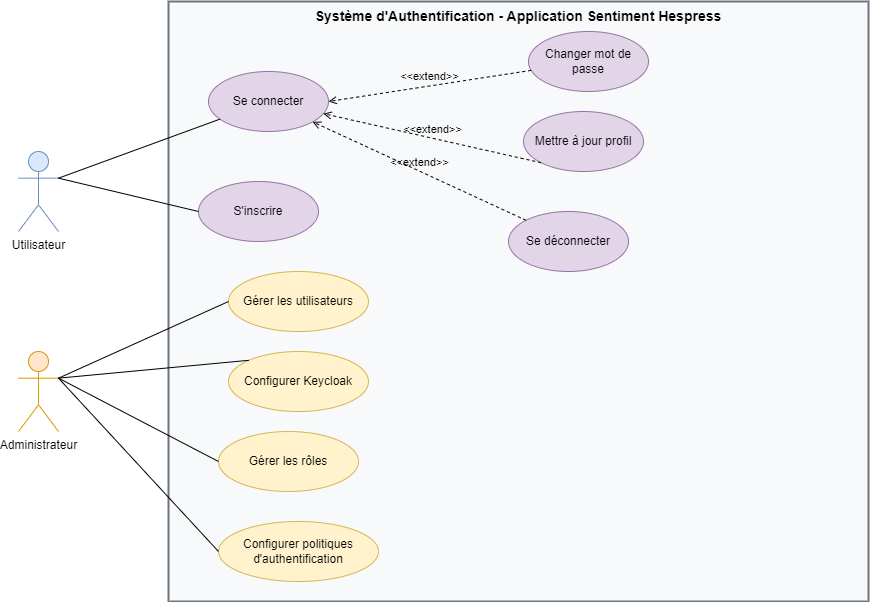
\includegraphics[width=0.8\textwidth]{assets/images/auth-usecase.png} 
\caption{Diagramme de cas d'utilisation du sprint 1 - Authentification}
\label{fig:sprint1-usecase}
\end{figure}

Ce diagramme illustre les interactions principales entre les acteurs (administrateur, utilisateur, développeur) et le système durant le premier sprint. Les cas d'utilisation se concentrent sur la configuration de l'environnement de développement et la mise en place du système d'authentification via Keycloak.

\subsection{Diagramme de Classe du Sprint 1}

\begin{figure}[H]
\centering
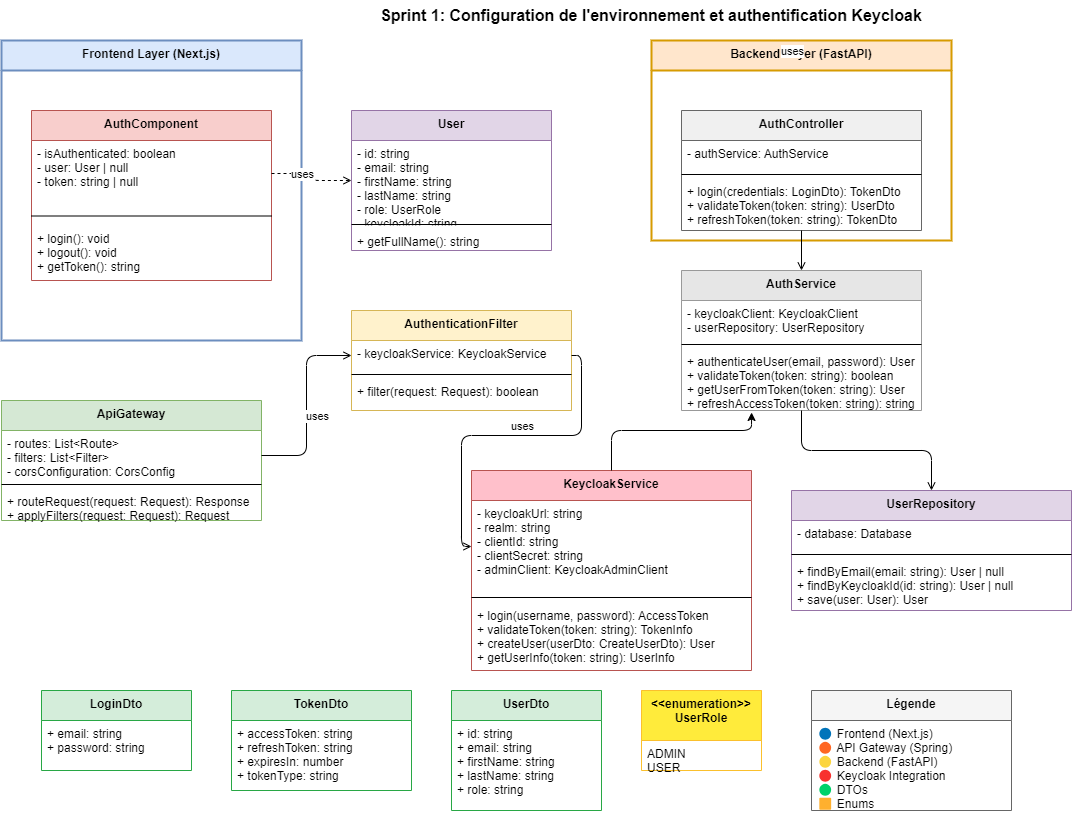
\includegraphics[width=0.9\textwidth]{assets/images/sprint1-class.png}
\caption{Diagramme de classe du sprint 1 - Architecture de base}
\label{fig:sprint1-class}
\end{figure}

L'architecture objet du sprint 1 met en évidence les classes principales : UserController, AuthService, GatewayConfig, et DatabaseConfig. Ces classes forment le cœur de l'infrastructure de base et du système d'authentification.

\subsection{Diagramme de Séquence de l'Authentification}

\begin{figure}[H]
\centering
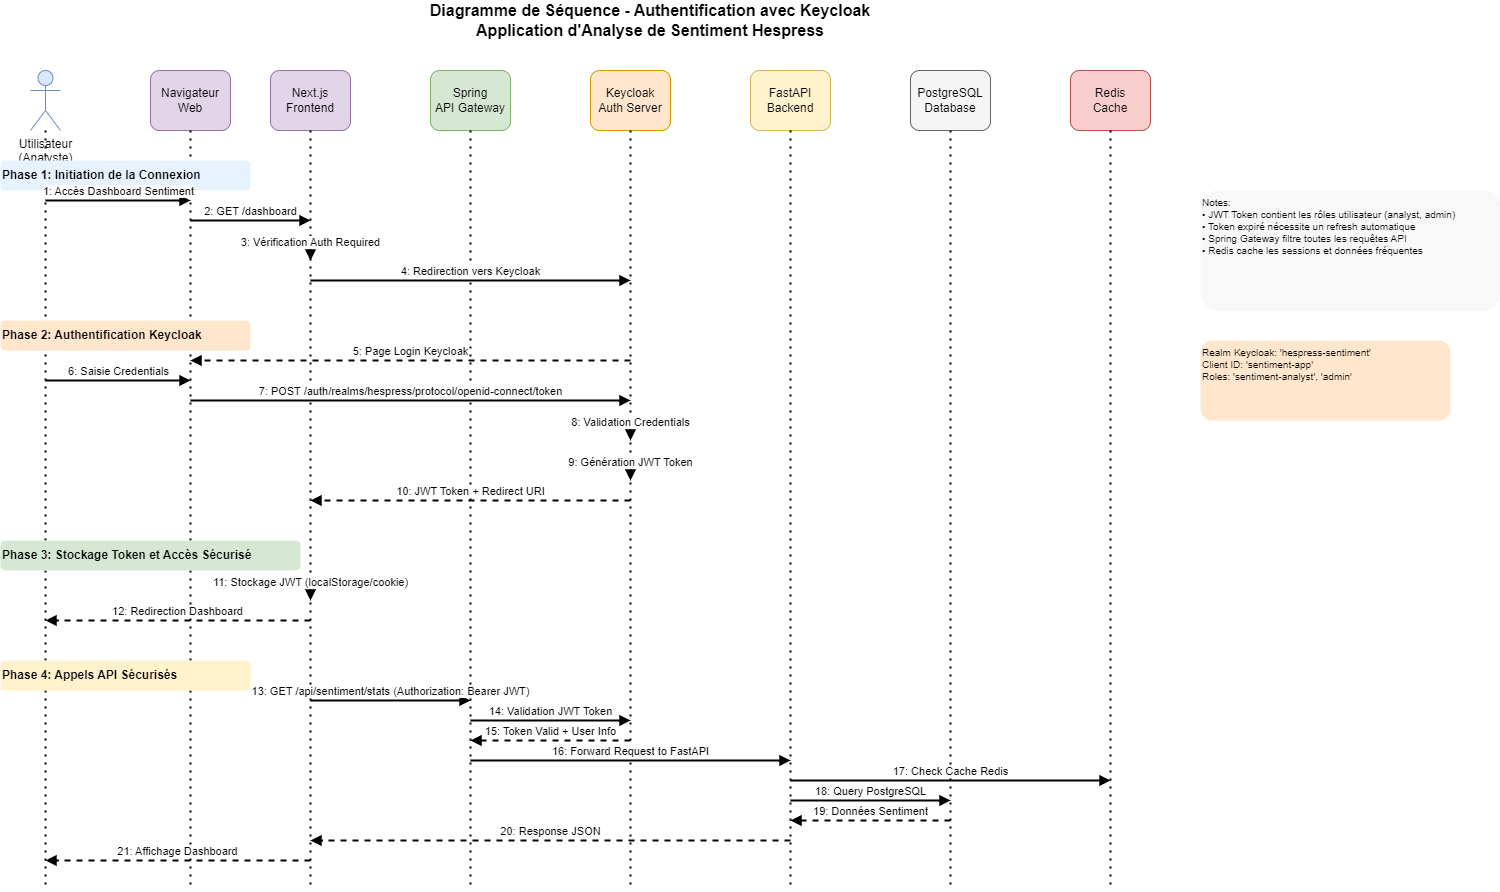
\includegraphics[width=0.9\textwidth]{assets/images/auth-sequence.png}
\caption{Diagramme de séquence du processus d'authentification}
\label{fig:auth-sequence}
\end{figure}

Ce diagramme détaille le flux d'authentification depuis la connexion utilisateur sur Next.js jusqu'à l'accès aux APIs sécurisées via Spring Gateway et FastAPI. Il montre l'orchestration entre Keycloak, Next.js, Spring Gateway et FastAPI pour garantir un accès sécurisé aux ressources.

\section{Réalisation du Sprint 1}

Le sprint 1 a abouti à la mise en place d'un environnement de développement complet et d'un système d'authentification fonctionnel. Les premières démonstrations ont validé la faisabilité technique et l'efficacité de l'intégration entre les différents composants.

\subsection{Interface d'Authentification}

L'interface développée avec Next.js offre une expérience utilisateur moderne et intuitive pour l'authentification. L'intégration avec Keycloak via NextAuth.js permet une connexion sécurisée avec support de différents providers d'authentification.

\subsection{Configuration de la Base de Données}

PostgreSQL a été configuré avec les schémas de base nécessaires pour le stockage des utilisateurs et des données d'authentification. Redis a été intégré pour la gestion des sessions et le cache des tokens JWT, améliorant les performances d'authentification.

\subsection{Sécurisation des APIs}

FastAPI a été sécurisé avec l'intégration des tokens JWT fournis par Keycloak. Spring Gateway agit comme point d'entrée unique, gérant l'authentification et l'autorisation avant de router les requêtes vers les services appropriés.

\subsection{Validation et Perspectives}

Le sprint 1 a posé les bases solides de l'infrastructure de développement, en validant les choix technologiques et en démontrant la faisabilité de l'architecture microservices. L'environnement de développement est maintenant prêt pour accueillir les fonctionnalités métier.

Les prochains sprints se concentreront sur le développement du module de web scraping avec Selenium, le prétraitement des données avec Pandas, et l'initialisation de l'API de récupération des données selon le plan de release défini.